\documentclass[11.5pt]{sig-alternate}
\usepackage[defaultlines=3,all]{nowidow}
\usepackage{tabularx}
\usepackage{graphicx}
\usepackage{blindtext}
\usepackage[utf8]{inputenc}
\usepackage[english]{babel}
\usepackage{lastpage}
\usepackage{comment}
\usepackage{dirtytalk}
\usepackage{xcolor}
\usepackage{hanging}
\usepackage{wrapfig}
\usepackage[backend=biber, style=apa]{biblatex}
\addbibresource{notation.bib}
\usepackage{authblk}
\usepackage{caption}
\usepackage{graphicx,subfigure}
\usepackage{authblk}
\usepackage{enumitem}
\usepackage[utf8]{inputenc}
\usepackage{cuted}
\usepackage{fancyhdr}
\usepackage{lipsum}
\usepackage{xurl}
\usepackage{hyperref}
\pagestyle{fancy}
\renewcommand{\headrulewidth}{0pt}
\renewcommand{\footrulewidth}{0pt}
\setlength\headheight{80.0pt}
\addtolength{\textheight}{-80.0pt}
\chead{%
  \ifcase\value{page}
  % empty test for page = 0
  \or 
\includegraphics[width=\textwidth]{headerImage.png}% page = 1
  \or 
\includegraphics[width=\textwidth]{headerImage.png}% page = 2
  \or 
\includegraphics[width=\textwidth]{headerImage.png}% page = 3
  \or 
\includegraphics[width=\textwidth]{headerImage.png}
  % page = 4
  \or 
\includegraphics[width=\textwidth]{headerImage.png}% page = 5
  \else
  
\includegraphics[width=\textwidth]{headerImage.png}
  \fi
}

%\chead{
\includegraphics[width=\textwidth]{headerImage.png}}
\fancyfoot[LE,LO]{One-Week Inquiry about Gravity Force with a Student Who is Blind\\
DOI:10.14448/jsesd.14.0007 }
\fancyfoot[CE,CO]{{ }}
\fancyfoot[RE,RO]{\thepage}
\pagenumbering{arabic}
\hypersetup{
    colorlinks=true,
    urlcolor=blue
}
 
\let\oldabstract\abstract
\let\oldendabstract\endabstract
\makeatletter
\renewenvironment{abstract}
{\renewenvironment{quotation}%
               {\list{}{\addtolength{\leftmargin}{1em} % change this value to add or remove length to the the default
                        \listparindent 1.5em%
                        \itemindent    \listparindent%
                        \rightmargin   \leftmargin%
                        \parsep        \z@ \@plus\p@}%
                \item\relax}%
               {\endlist}%
\oldabstract}
{\oldendabstract}
\makeatother

% Left align captions
\captionsetup{justification   = raggedright,
              singlelinecheck = false}


\begin{document}

\title{One-Week Inquiry about Gravity Force \\with a Student Who is Blind}

\author[1]{\large \color{blue}Mustafa Şahin Bülbül}

\affil[1]{	Assistant Professor at Kafkas University}

\toappear{}

\maketitle
\begin{@twocolumnfalse} 
\begin{abstract}
\begin{large}
\item 
 \textit {This study was conducted with a student who is visually impaired and questioned the force of gravity. The different stages encountered in the process were specified as steps in the study and it was shared what kind of inquiry form was needed at each step. There are different activities such as waiting for a week and thought experiment in the inquiry activity. The basis of the activity is that three balls of different mass left on a sponge leave different traces on the sponge.}
     \\
     \\
     \textbf{Keywords:} Inquiry, Long Term Projects, Gravity Force
\end{large}
\end{abstract}
\end{@twocolumnfalse}

%% ABSTRACT


%% AUTHOR INFORMATION

\textbf{*Corresponding Author, Mustafa Şahin Bülbül }\\
\href{mailto: msahinbulbul@gmail.com }{(msahinbulbul@gmail.com)} \\
\textit{Submitted December 2 2022 }\\
\textit{Accepted December 12 2022} \\
\textit{Published online December 21 2022} \\
\textit{DOI:10.14448/jsesd.14.0007} \\


\pagebreak
\pagebreak

\vspace{5mm}
\section*{\vspace{140mm}}
\begin{large}

\section*{Introduction}
The gravitational force is a force that we do not see with our eyes, but that we know exists and that we sometimes feel due to changes. For example; What we feel during takeoff and landing while inside the plane is related to the change in the net force acting on us, and the gravitational force also has an effect on this change. We also remember the force of gravity when we see something sinking or falling to the ground, apart from the emotions we feel on the plane and in the elevator. How can this force towards the center of the earth be investigated by a student who is blind?

Inquiry can be applied in large-scale classrooms (Scherr, 2003) as well as in individual studies (González-Espada, 2012). This individual may even be a student who is blind. The student who is blind needs to be involved by using his/her senses other than sight, namely auditory and tactile senses. In this research, a long-term inquiry activity will be presented, which is liked, thought to be fun, stated to contribute to her learning, and tried with a high school student who is visually impaired.

It is known that not every hands-on activity is inquiry (Blanton, 2007). The main purpose of inquiry studies is to make students think more deeply (Alake-Tuenter, Biemans, Tobi, Wals, Oosterheert \& Mulder, 2012; Haegele, Sato, Zhu \& Avery, 2017). For this purpose, it is possible to adapt the classroom environment and materials for students who are blind and to have them discussed in a group (Villanueva \& Di Stefano, 2017), as well as to extend the time used and focus on a student's thoughts that are not influenced by others. 

The inquiry work was carried out in three main phases and a total of ten steps. All these steps have been designed to contribute to the understanding of the nature of science and scientific process skills, as well as to reflect on the concept. A student who is visually impaired and a researcher were found at each step. The ten basic steps, which were formed by preserving the three basic phases, were changed according to what the student in the process was curious about and wanted to do. Therefore, the shared ten-step inquiry process was created as a result of a natural learning flow with a high school student who is visually impaired.

\section*{Phase 1: Before the wait}

\subsection*{\textit{Step-1: Identify materials}}

The student needs to get to know the materials before the materials interact. Before talking about the material, the material should be given and the student should be able to examine the material by touching it. If he asks a question, he should be answered when he is sure that the examination is completely over, otherwise, there may be a loss between the tactile data and the spoken verbal data. If the student does not ask any questions, you can make an introductory explanation of the materials. Try not to make too many explanations other than the statement ``There are three balls of different masses in front of you and a piece of sponge on which you can put the balls (Figure 1)".

\begin{figure}[h]
    \centering
    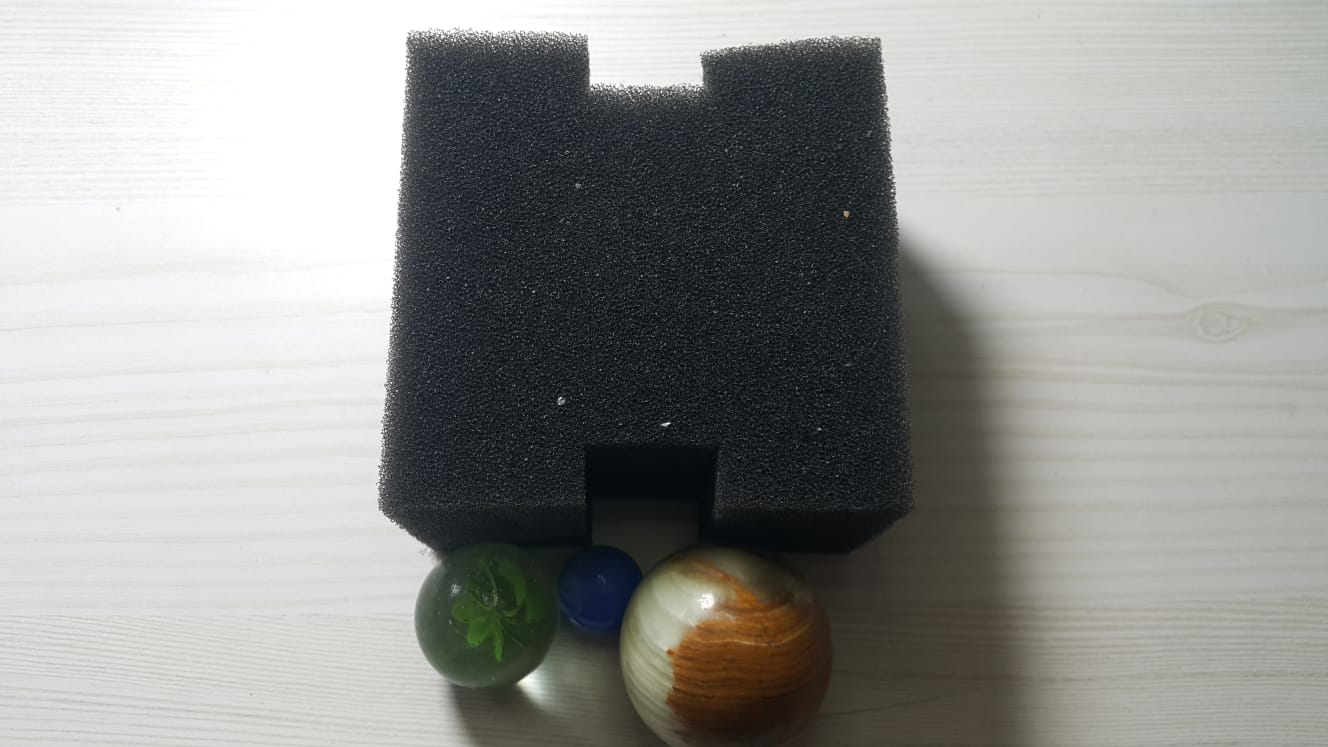
\includegraphics [width=\columnwidth]{Figure1.png}
    \captionsetup{font=large, labelfont=bf}
    \caption{Elements of the inquiry setup; three different balls and a piece of sponge}
    \label{Figure 1}
\end{figure}

\subsection*{\textit{Step-2: What would you like to do?}}
Before telling the student what to do, it is necessary to make him think about his thoughts. Reflecting on the student's thoughts will increase their awareness of the inquiry process. For this purpose, he asked her, ``What would you like to do with these materials?" It is necessary to continue the activity by asking. While the student is telling what he/she wants to do with the materials, it is necessary not to give right or wrong directions. At this stage, the student has completed his awareness of the materials and is ready to think deeply about them. If the proposal is a short-term proposal that can be made and will not disrupt the structure of the activity, you should not hesitate to make it. If it is a long-term suggestion that will harm the materials, you should tell him that you will give these materials to him at the end of the event and that he can try this suggestion. The student whose suggestion is allowed to be made will be easily persuaded to make the teacher's activity suggestion.

\subsection*{\textit{Step-3: Guess what will happen}}
If the student is motivated to make your proposal, you can now share your inquiry proposal and ask your student if they would like to make it. Tell your student that you are going to put the marbles on the sponge and wait a week and see what will change. If your student starts sharing their guesses, you are in step three. You can make the student think at this step with questions such as: ``What changes will happen to the marbles and the sponge at the end of a weekend, will the changes (eg. scars) be different from each other?" 

\section*{Phase 2: The wait}

\subsection*{\textit{Step-4: Start the experiment}}
Now the student is ready for the fourth step where the activity will start. He needs to see the result of his guess and learn whether he guessed correctly. For this, the student will wait as long as a week. Have the student take the marbles and put them on the sponge with their own hands. Remind him not to forget how he put it and the position of the marbles. Do not forget to indicate to the student that you will make an effort not to damage the device. Since the student and the teacher cannot wait at the beginning of the mechanism all the time, some precautions should be taken. For example, if the position of the balls has changed, someone may have intervened in the mechanism. Such reliability measures are experiments, and thus approaches inherent in science. Conducting the event as designed is extremely important for a healthy assessment.

\subsection*{\textit{Step-5: Keep inquiry one week}}
After making sure that three balls of different mass are placed on the sponge (Figure 2) and stored securely, ask the student to think about the question you asked in step three for a week. As you meet, it should be learned whether he ``has a new thought" by reminding the question to your student in phone calls and instant messages.

\begin{figure}[h]
    \centering
    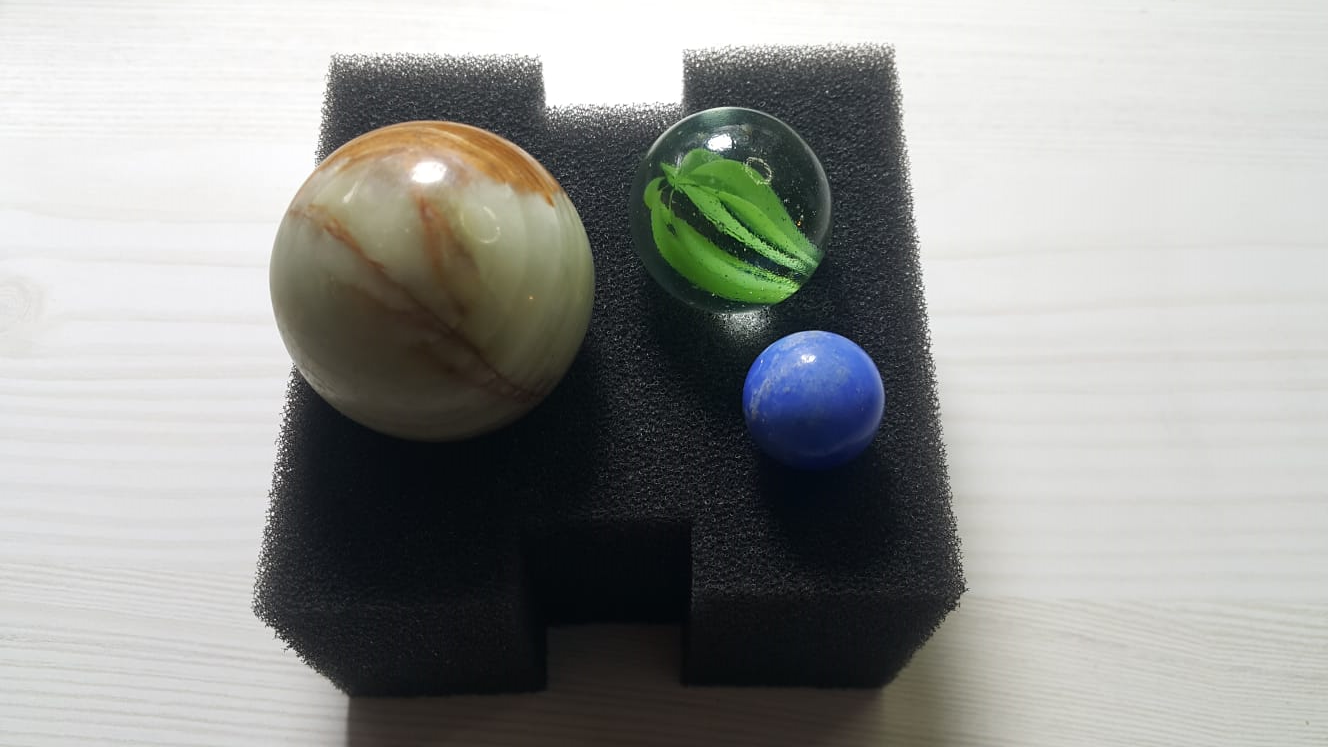
\includegraphics [width=\columnwidth]{Figure2.png}
    \captionsetup{font=large, labelfont=bf}
    \caption{The setup during the wait}
\end{figure}

In this step, our student is visually impaired informed us that she thought ``I wonder if there will be a change in the shape of the marbles". She came to the conclusion that the shape of the marbles would not change, but we recorded it as a situation that he had to control. At the end of a week, it was decided to check not only the trace expected to form on the sponge, but also the trace that was not expected to form on the marble.
 
\section*{Phase 3: After the wait}

\subsection*{\textit{Step-6: Check the setup}}
Before answering the question that has been thought about for a week without touching the device, the student should make sure that the device is as he left it. This control is important for the reliability of the comments to be made. In addition to the teacher's control, it is extremely important for the student to check himself and express that the mechanism is not broken. The situations that the student suspects should be clarified and one should not proceed to the next step without being completely sure. 

\subsection*{\textit{Step-7: Examine the change}}
The marbles should be lifted slowly and carefully by the student. We assume that questions such as "Should we remove the marbles one at a time or do we remove them all at once" are decided during a week of inquiry. According to the decision, both the traces on the sponge and the size of these traces and the traces on the balls (if any) should be examined. A change in the shape of the ball will not be noticed. Also, the student may want to hold the marbles, give them to you, or put them in a container. It is necessary to assist the student in the process. In our research, our student wanted to lift each marble himself and check both the trace on the marble and the trace on the sponge (Figure 3). She started with the largest one in order and searched for the smallest marble to the last. After they were all done, he wanted to compare the tracks and gave the marbles to the researchers.

\begin{figure}[h]
    \centering
    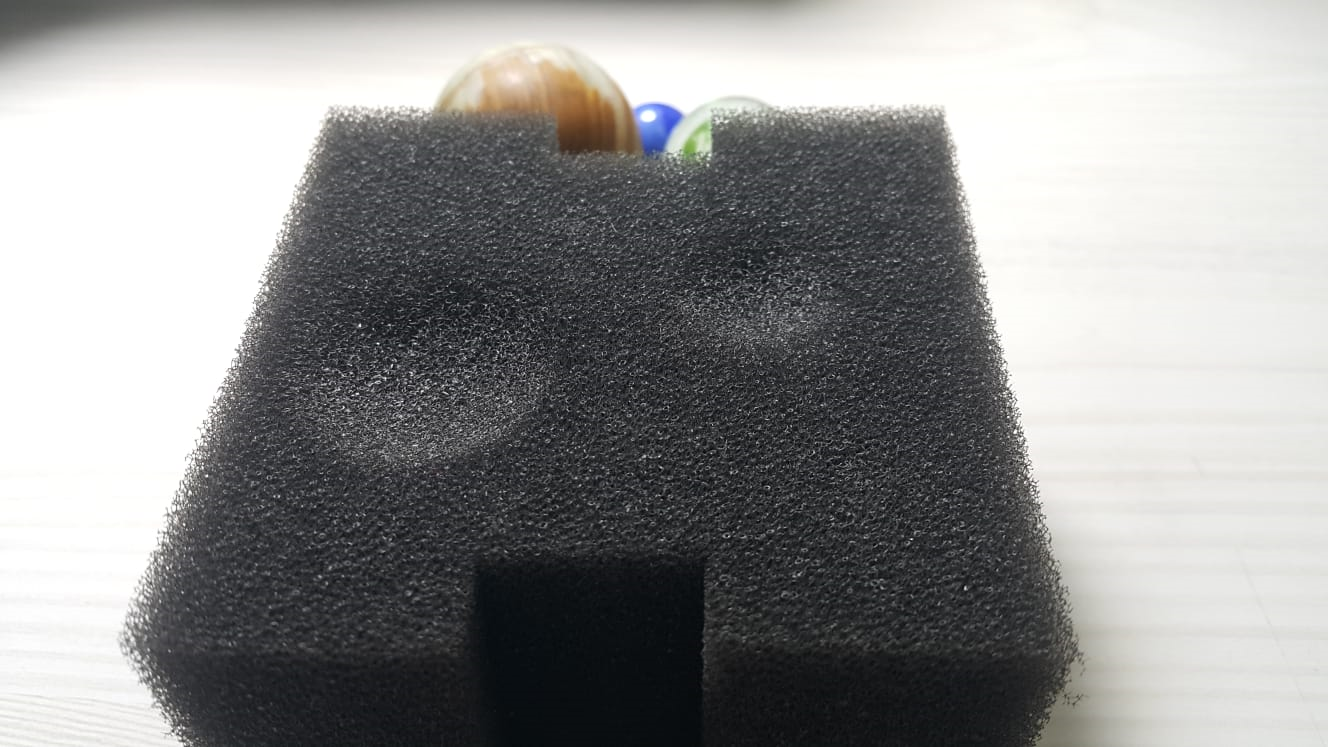
\includegraphics [width=\columnwidth]{Figure3.png}
    \captionsetup{font=large, labelfont=bf}
    \caption{The result of one-week inquiry setup}
\end{figure}


The student who is blind could not detect the trace of the smallest marble by touch. Although he could not perceive it, the student argued that there must be a trace under the marble, even if it is very small. The reason for this thought was the experience of ``balls make traces in proportion to their masses". This encounter was an important experience regarding the inconsistency between theory and practice and measurement errors related to the nature of science and scientific process skills.
 
\subsection*{\textit{Step-8: Think about the change}}
The track created by the massive ball was both larger in diameter and greater in depth. For this reason, it can be concluded by the student who is blind that the ball exerts a greater force on the sponge as the mass increases. The elastic structure of the sponge can produce a force that will absorb the effect of the small force applied, but the damaging effect of large-mass objects prevents the sponge from recovering. 
 
\subsection*{\textit{Step-9: Connect with life}}
After some inferences that the student will make, they need to verify these inferences with examples from daily life. For example, the student should be able to answer the question of whether large rocks or small stones will create a greater depth in the soil, in the light of his experience. The student who is visually impaired we worked with shared that he thinks that when the footprints of animals are examined, the larger ones can show deeper footprints
 
\subsection*{\textit{Step-10: Think on other contexts}}
Having focused on the activity, thinking for a week, and experiencing the results, the student is now ready to experiment with other contexts. thought experiment; It includes experiments that can be done by thinking only, without entering the laboratory. The important thing in thought experiments is to generalize from extreme examples. For this activity, we asked our student who is visually impaired what would be the result if we used materials such as ``iron, wood, water and air". He said that the balls left in the air will fall until we hold them, but they will leave small traces on the iron that we cannot notice with our hands, but if he puts a ball with a larger mass, this time we can also feel the trace on the iron. One of the most important implications was their statement that force should be an ongoing concept as long as mass. The gravitational force had to continue to act for a week so that those marks could form.

\section*{Conclusion}
As everyone knows, in environments where there is no air resistance, two different masses that are left to fall freely fall to the ground at the same time. This is because the gravitational acceleration of the same magnitude affects both masses. Therefore, different forces act on different masses. In this study, we see different-sized traces formed due to the different-sized masses of marbles with very close densities. Simply by touching, we can realize that the Earth attracts a large mass with great force. For further study, the density of the sponge, the surface and depth of the trace (volume of the sinking part), and balls of different densities can be used. 

Inquiry, by its very nature, requires deep thinking and therefore the need for additional time. Ten steps naturally formed at the end of this inquiry activity, which is tactilely designed to enable student who is blind to meditate on an abstract topic such as the force of gravity, are shared in this study. Teachers need to focus on ways to deepen thinking with simple materials, avoiding the worry of not being able to teach scientific concepts to a student who is blind. Having a student who is blind is not just bad luck, but perhaps an opportunity to expand your experience in a student who is blind, thought-centered activities such as inquiry and thought experiments. In thought experiments, you need words to describe the situation, not the test tubes or electrical wires. Touching and describing, two ways of communicating through inquiry with a student who is blind, were used together in this activity. The fact that teachers make their activities descriptive and tactile actually means that they appeal more to the senses, which creates lessons in inclusive environments in which all students can be involved.

\include{} 
\section*{References}\par 

\leftskip 0.25in
\parindent -0.25in 
Blanton, P. (2007). Developing an inquiry lesson. \textit{The Physics Teacher, 45}(1), 56-57.\\

Scherr, R. E. (2003). An implementation of Physics by Inquiry in a large-enrollment class. \textit{The Physics Teacher, 41}(2), 113-118.\\

González-Espada, W. J. (2012). Falling PC Solitaire Cards: An Open-Inquiry Approach. \textit{The Physics Teacher, 50}(6), 365-366.\\

Villanueva, I., \& Di Stefano, M. (2017). Narrative inquiry on the teaching of STEM to blind high school students. \textit{Education Sciences, 7}(4), 89.\\

Haegele, J. A., Sato, T., Zhu, X., \& Avery, T. (2017). Physical education experiences at residential schools for students who are blind: A phenomenological inquiry. \textit{Journal of Visual Impairment \& Blindness, 111}(2), 135-147.\\

Alake-Tuenter, E., Biemans, H. J., Tobi, H., Wals, A. E., Oosterheert, I., \& Mulder, M. (2012). Inquiry-based science education competencies of primary school teachers: A literature study and critical review of the American National Science Education Standards. \textit{International Journal of Science Education, 34}(17), 2609-2640.

\end{large}
\end{document}
